\hypertarget{convdiff2D_8cpp}{
\subsection{/home/luiggi/Documents/Research/Meshless\_\-RBF/NEW/RBFSoft/examples/05ConvDiff2D/convdiff2D.cpp File Reference}
\label{convdiff2D_8cpp}\index{/home/luiggi/Documents/Research/Meshless\_\-RBF/NEW/RBFSoft/examples/05ConvDiff2D/convdiff2D.cpp@{/home/luiggi/Documents/Research/Meshless\_\-RBF/NEW/RBFSoft/examples/05ConvDiff2D/convdiff2D.cpp}}
}
Forced Convection in 2D.  




\subsubsection{Detailed Description}
Forced Convection in 2D. 

In this example the time-dependent convection-diffusion equation is solved. The equation is written as follows: \[ \frac{\partial T}{\partial t} + u \frac{\partial T}{\partial x} + v \frac{\partial T}{\partial y} = \Gamma\left( \frac{\partial^2 T}{\partial x^2} + \frac{\partial^2 T}{\partial y^2} \right)\] where $(u, v)$ is a prescribed velocity field that fulfills the continuity equation and is given by the next formula: \begin{eqnarray*} u(x,y) & = & -A\cos(\pi y) \sin(\pi \lambda x / l_x ) \mbox{and} \\ v(x,y) & = & \frac{A \lambda}{l_x} \sin(\pi y) \cos(\pi \lambda x / l_x). \end{eqnarray*} The initial condition is $T=0$ and the boundary conditions are as shown in the next figure:  \begin{Image}
\begin{center}
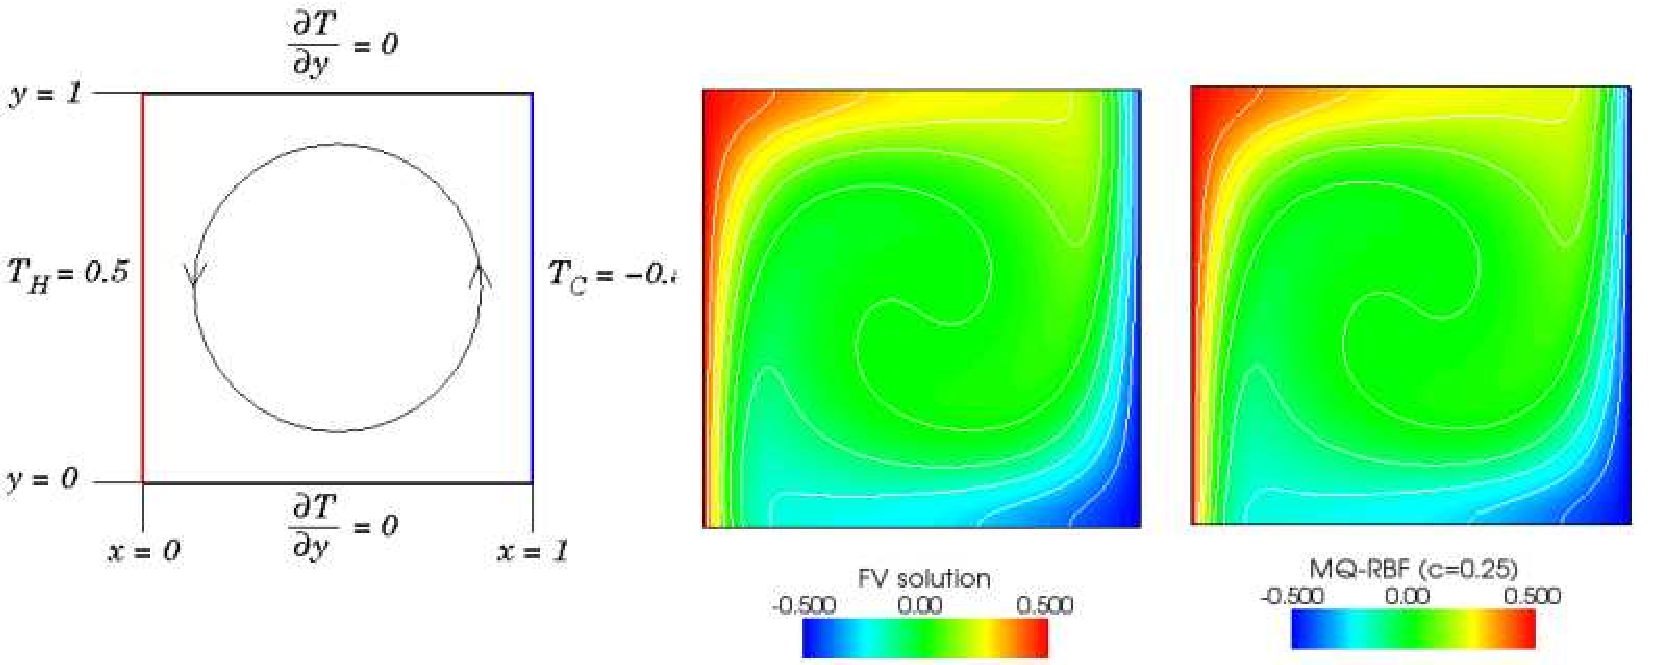
\includegraphics[width=5cm]{solconv2D}\caption{Geometry, boundary conditions and solution}
\end{center}
\end{Image}
 \begin{Desc}
\item[Input]The {\tt input} file contains the initial data to setup the problem.\begin{itemize}
\item {\tt hx}, {\tt hy}, {\tt Nx}, {\tt Ny} : Lenghts of the rectangle, and number of points in each axis.\item {\tt rtype}, {\tt ep}, {\tt layer} : Type of knots distribution, randomness, layer around the domain.\item {\tt max\_\-iter} time iterations, {\tt dt} Step time step\item {\tt max\_\-knots} : neighbors used to construct the ACBF preconditioner.\item {\tt c} : Shape parameter for MQ-RBF kernel ($c < 0$ implies $ c = 1/\sqrt{N}$).\item {\tt cboundary} : Shape parameter for MQ-RBF kernel on the boundary ($c < 0$ implies $ c = 1/\sqrt{N}$).\item {\tt A} max magnitude of the velocity.\item {\tt Nprofile} number of points to make the velocity profiles. \end{itemize}
\end{Desc}
\begin{Desc}
\item[Output]\begin{itemize}
\item {\tt xy\_\-knots.dat} coordinates of random points;\item {\tt solution.dat} (x,y,u) evaluation of the solution in a grid.\item {\tt profBF\_\-x.dat}, {\tt profRBF\_\-y.dat} velocity profiles through the middle of the cavity.\end{itemize}
\end{Desc}
\begin{Desc}
\item[Author:]Luis M. de la Cruz Wed \mbox{[} Dec 19 14:49:56 GMT 2007 \mbox{]} \end{Desc}


Definition in file \hyperlink{convdiff2D_8cpp-source}{convdiff2D.cpp}.